\section{Placa de circuito impreso del módulo exterior}
\label{app:componentes-exterior}

\subsection{Lista de materiales}

\vfill

\begin{table}[H]
\caption{Lista de materiales del módulo exterior (placa)}
\label{tab:materiales-circuito-exterior}
\begin{tabularx}{\textwidth}{cX}
\toprule
\headingc{Cantidad} & \headingc{Descripción} \\
\topruleb
  1 & PCB de prototipado (70mm x 90mm)\\*\midrule
  1 & NodeMCU v3 (ESP8266)\\*\midrule
  1 & 1 sensor DHT22 (placa)\newline(Nota: la figura~\ref{fig:exterior-pieces} muestra un sensor DHT11)\\*\midrule
  1 & Regulador de baja caída AP7361C-33ER-13\\*\midrule
  1 & Botón \textit{push} (normalmente abierto)\\*\midrule
  1 & Portabaterías 4 pilas AA \\*\midrule
  1 & Interruptor de flotador (normalmente cerrado)\\*\midrule
  1 & Resistencia 100 kΩ \\*\midrule
  1 & Resistencia 220 kΩ \\*\midrule
  1 & Interruptor de dos posiciones (3 pines)\\*\midrule
 -- & Pines variados\\*\midrule
 -- & Conectores Dupont variados\\*\midrule
 -- & Cables variados\\*\bottomrule
\end{tabularx}
\end{table}

\vfill

\clearpage

\begin{sidewaysfigure}
  \centering
  \includegraphics[width=0.98\columnwidth]{../photos/exterior-pieces}
  \caption{Piezas para la construcción del módulo exterior}
  \label{fig:exterior-pieces}
\end{sidewaysfigure}

\clearpage

\subsection{Diseño de circuito impreso del módulo exterior}

\importantbegin{Modificación del hardware}
El \MEE emplea una placa NodeMCU v3 (ESP8266) modificada. Obsérvese en el centro de la figura~\ref{fig:exterior-board-front} (marcado en gris) que el regulador de voltaje que monta la placa NodeMCU v3 por defecto (AMS1117) ha sido retirado y sustituido por un regulador de baja caída AP7361C-33ER-13 con la misma disposición de pines y menor consumo en reposo (60 $\mu$A).

\textbf{El regulador AP7361C-33ER-13 admite voltajes de entrada entre 2,2 V y 6,0 V, por lo que no es posible emplear 4 pilas alcalinas en el \MEE.}
\importantend


\begin{figure}[H]
  \centering
  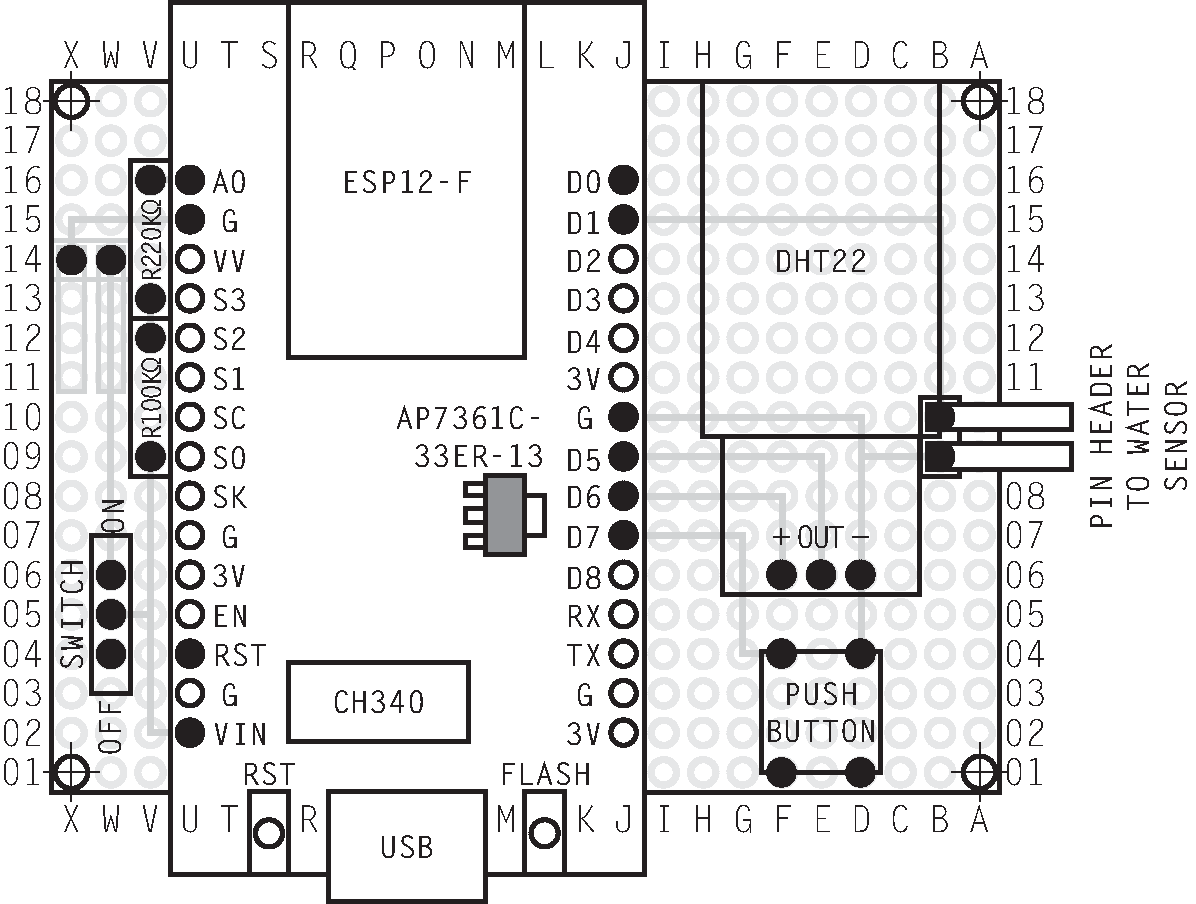
\includegraphics[width=0.9\columnwidth]{../design/exterior-board-front}
  \caption{Diseño frontal de la placa de circuito impreso}
  \label{fig:exterior-board-front}
\end{figure}

\vfill

\clearpage

\begin{figure}
  \centering
  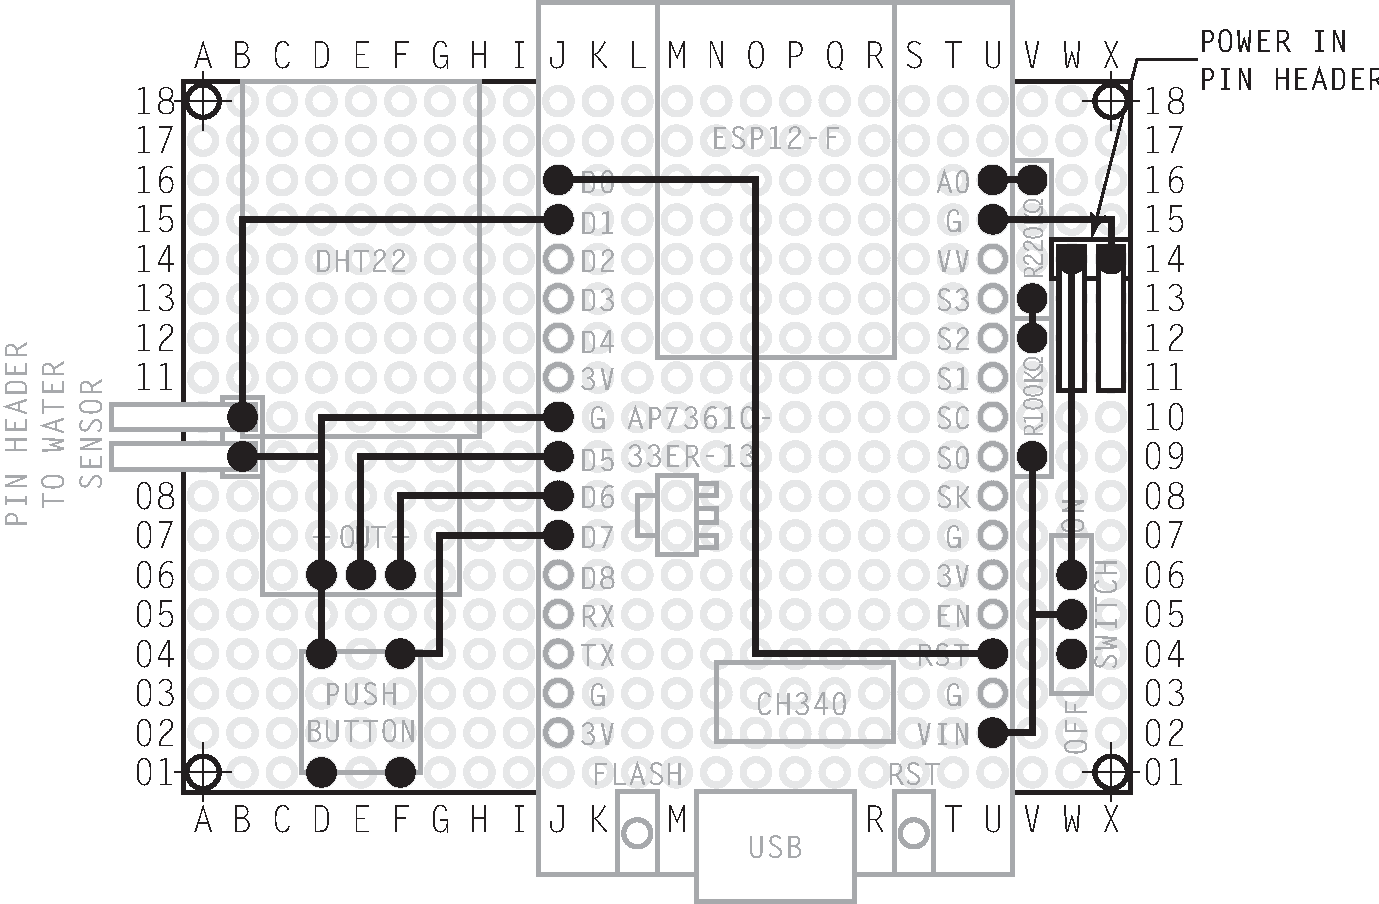
\includegraphics[width=0.9\columnwidth]{../design/exterior-board-back}
  \caption{Diseño trasero de la placa de circuito impreso}
  \label{fig:exterior-board-back}
\end{figure}

\clearpage

\subsection{Acabado final}

\vfill

\begin{figure}[H]
  \centering
  \includegraphics[width=1\columnwidth]{../photos/exterior-pcb-front}
  \caption{Acabado final de la placa de circuito impreso (vista frontal)}
  \label{fig:exterior-pcb-front}
\end{figure}

\vfill

\clearpage

\begin{figure}
  \centering
  \includegraphics[width=1\columnwidth]{../photos/exterior-pcb-back}
  \caption{Acabado final de la placa de circuito impreso (vista trasera)}
  \label{fig:exterior-pcb-back}
\end{figure}

\clearpage

